Le principe d'inductance ramenée explique le fait que lorsque la longueur du fil correspond au quart de la longueur d'onde, l'onde émise se voit
presque annulée en amplitude (car réduite par sa propre réflection). Cela veut donc dire que le fil mesuré est le fil ouvert.

\begin{equation}
    L = \frac{\lambda}{4}
    \label{eq:longueur4lambda-fréquentiel}
\end{equation}

 En utilisant la formule suivante, on peut calculer la longueur du fil si l'on connait la vitesse de transmission dans notre fil et la fréquence:

\begin{equation}
\lambda = \frac{v}{F} \label{eq:equation-vitesse-fréquentiel}
\end{equation}

 on peut donc combiner les équations \ref{eq:longueur4lambda-fréquentiel} et \ref{eq:equation-vitesse-fréquentiel} et le fait que nos fréquences
 seront en MHz et que notre vitese est une constante \ref{vitesse-transmission} afin d'obtenir la simple équation suivante:

 \begin{equation}
    \begin{aligned}
        \lambda & = \frac{2*10^8}{F*10^6} \\
        L & = \frac{200}{F} / 4 \\
        L & = \frac{50}{F}
        \label{eq:equation-longueur-simple}
    \end{aligned}
 \end{equation}

 Donc, en utilisant les résultats suivants obtenus en prenant la mesure de la fréquence lorsque l'amplitude est la plus réduite possible, comme
 la figure ci-dessous le démontre, on peut arriver aux résultats suivants.

\begin{figure}[H]
   \centering
   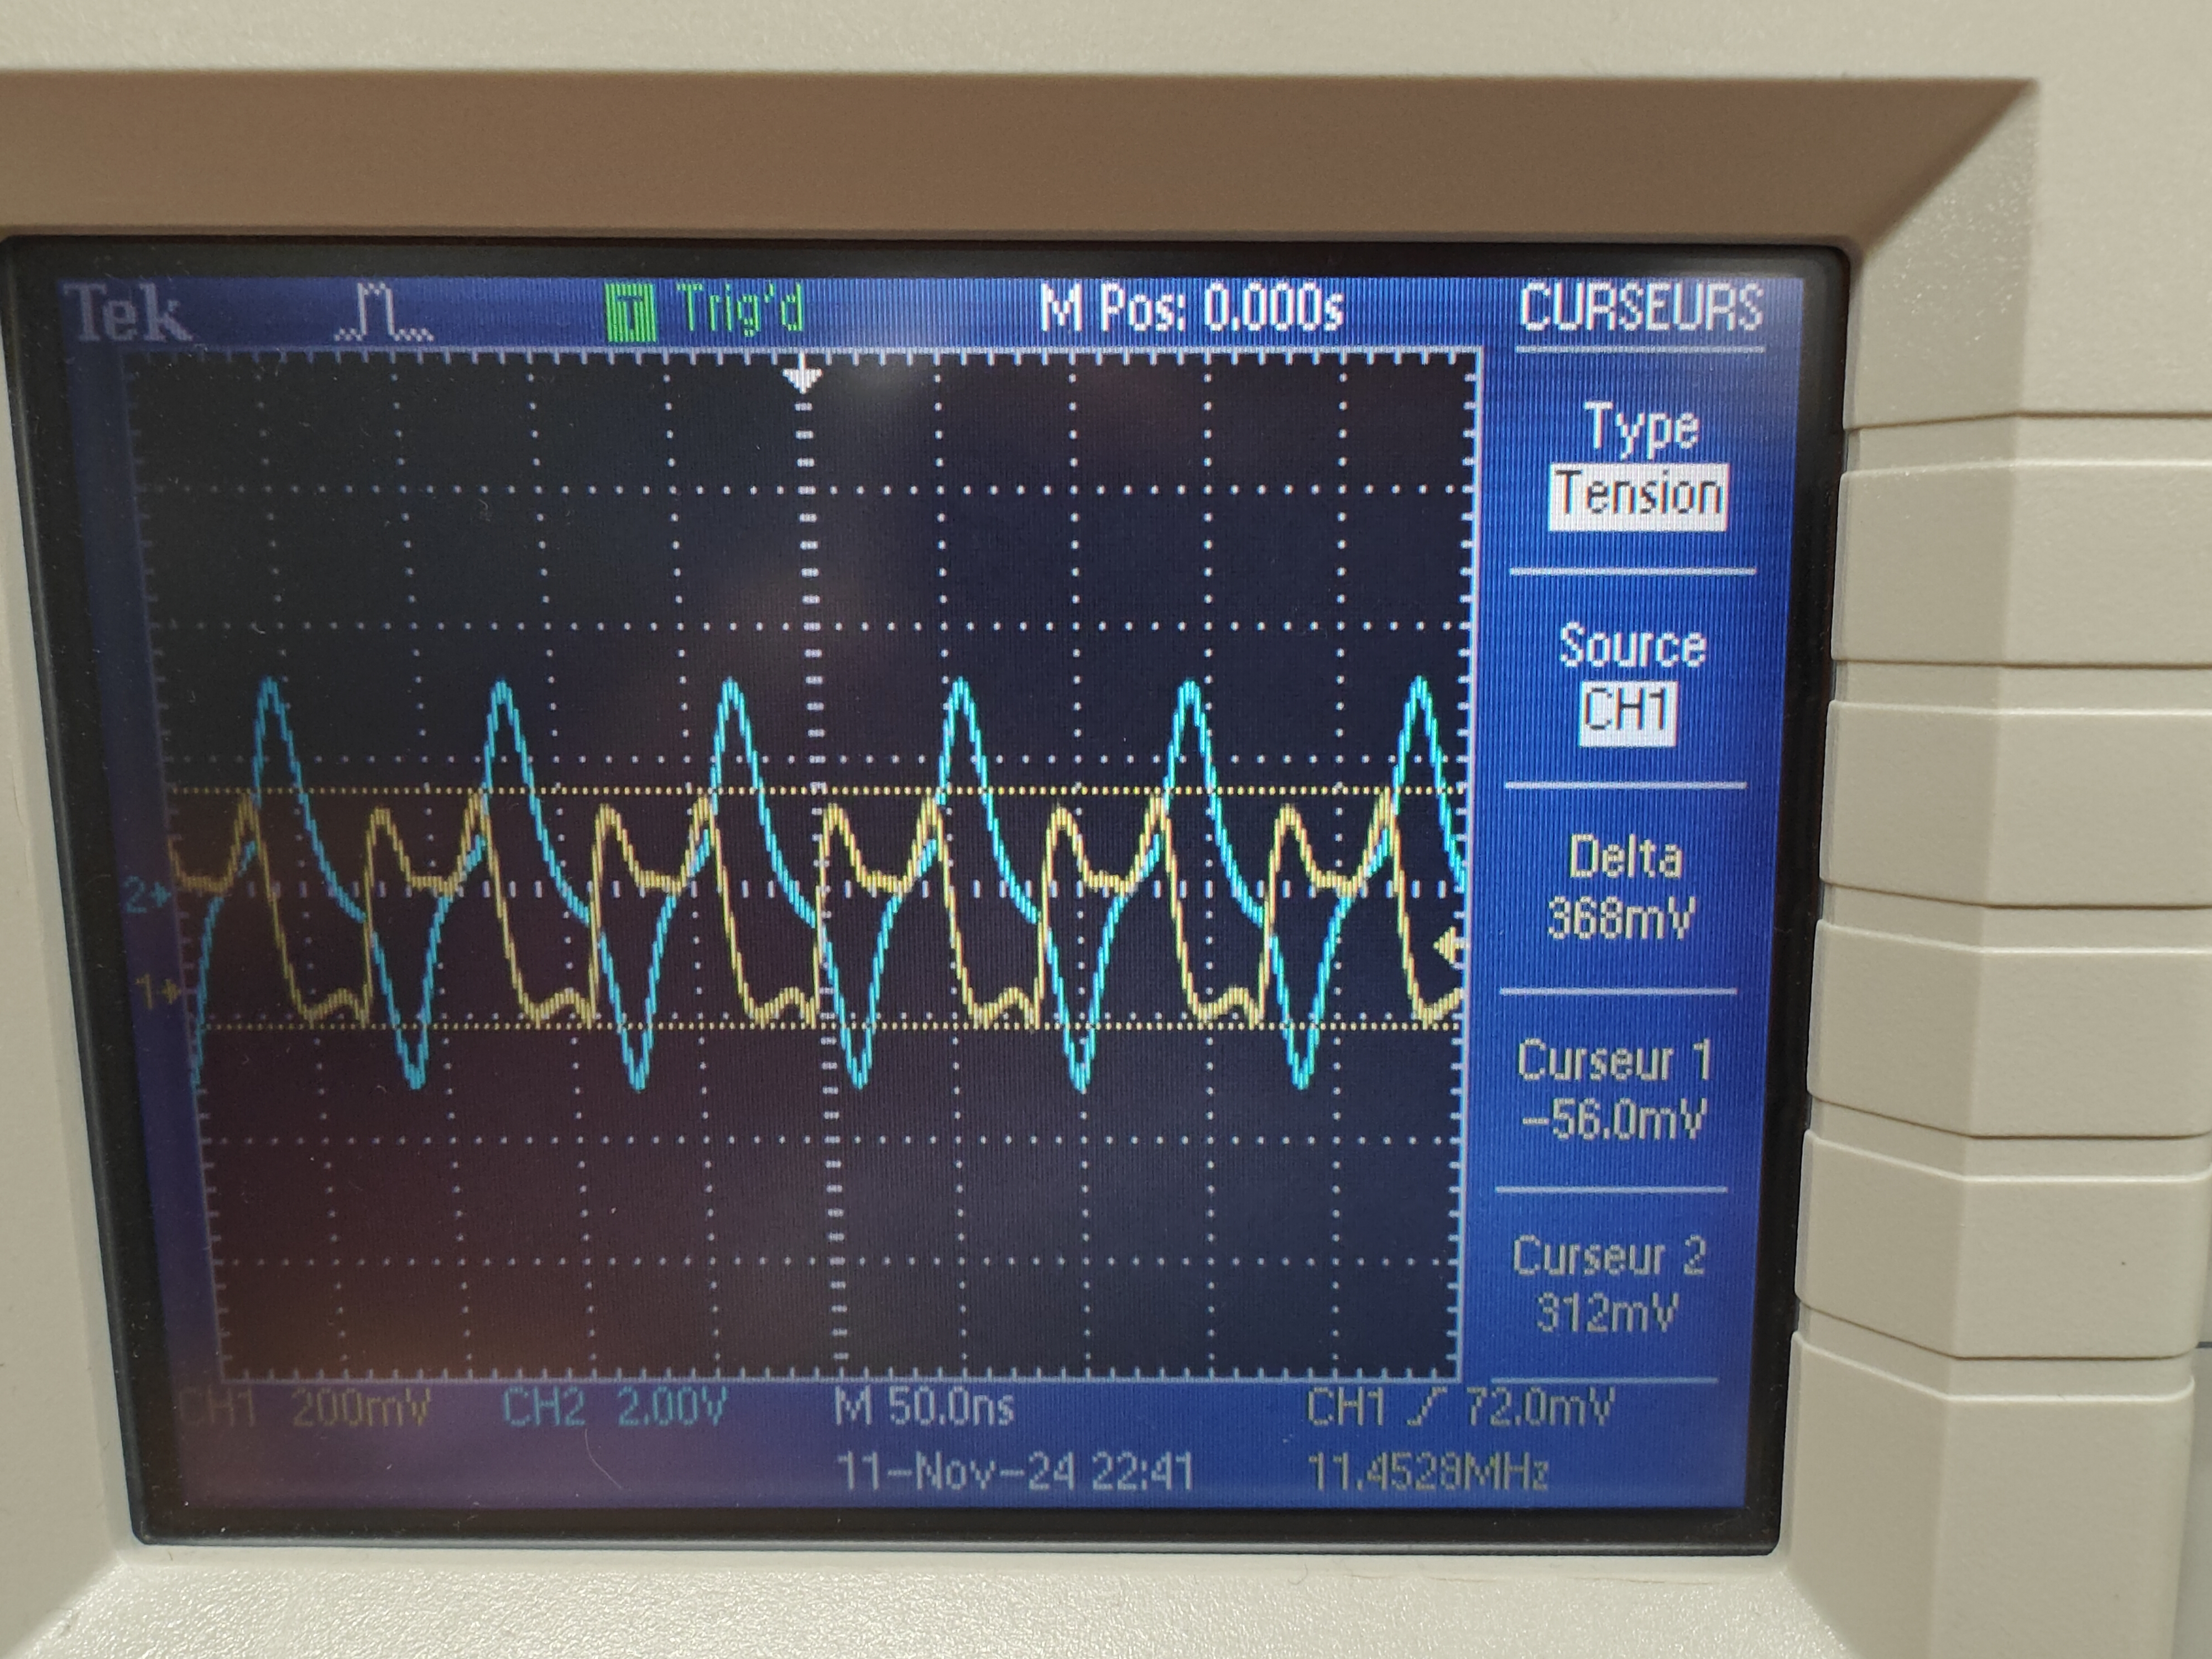
\includegraphics[width=0.7\textwidth]{images/c-frequentiel.jpg}
   \caption{Mesure fréquentielle d'aténuation du signal}
   \label{fig:mesure-frequentiel}
\end{figure}


\begin{center}
\begin{table}[H]
\caption{Résultats des mesures fréquentielles} \label{tab:tableau mesures fréquentiel}
\begin{tabularx}{\textwidth}{ X X X X }
   Fil d'entrée & Fil d'extrémité & Fil ouvert & Résultat (MHz) \\
   \hline
   \hline
    B & C & A & 8.18\\
    C & A & B & 6.5\\
    A & B & C & 11.45\\
    \hline
\end{tabularx}
\end{table}
\end{center}

On peut donc obtenir les résultats suivants en utilisant nos mesures et la formule de vitesse \ref{eq:equation-vitesse} on obtient 3 équations
et 3 inconnues.

\begin{center}
\begin{table}[H]
\caption{Longeurs selon les mesures fréquentielles} \label{tab:tableau longueur frequentiel}
\begin{tabularx}{\textwidth}{ X X }
    Fil & Longueur (m) \\
    \hline
    \hline
    A & 6.11 \\
    B & 7.69 \\
    C & 4.40 \\
    \hline
\end{tabularx}
\end{table}
\end{center}

On peut donc voir que les mesures concordent avec celles obtenues en \ref{tab:tableau longueur temporel}